\section{Problemi considerati}
\subsection{Alcune definizioni fondamentali della teoria dei grafi}
Riportiamo la definizione di \textit{relazione binaria} su uno o due insiemi, che sarà utile per definire formalmente il concetto di \textit{grafo}, che sarà fondamentale all'interno di questo elaborato.
\begin{definition}
    Chiameremo \textit{relazione binaria} su $A,B$ qualsiasi sottoinsieme del prodotto cartesiano $A \times B$.\\
    Chiameremo \textit{relazione binaria} su $A$ qualsiasi sottoinsieme del prodotto cartesiano $A \times A$.\\
    Diremo che $u,v$ sono \textit{in relazione} rispetto a $b$ se $(u,v) \in b$. In questo caso useremo la notazione $u b v$.
\end{definition}
Ad una relazione binaria su un insieme è possibile associare relazioni binarie che la contengono, le cosiddette \textit{chiusure}.
Ogni chiusura è costituita dall'unione della relazione iniziale e di un insieme di coppie costruito con un criterio differente a seconda del tipo di chiusura.\\
Quest'ultimo insieme fornisce la proprietà che caratterizza la chiusura (riflessività, simmetria, transitività).
\begin{definition}
    Sia $b$ una relazione binaria su $N$.
    Diamo le seguenti definizioni
    \begin{itemize}
        \item \textit{Chiusura riflessiva}: $b_r = b \cup \{(x,x) \,\, \forall x \in N\}$
        \item \textit{Chiusura simmetrica}: $b_s = b \cup \{(y,x) \,\, \forall x,y : (x,y) \in b\}$
        \item \textit{Chiusura transitiva}: $b_t = b \cup \{(x,z) \,\, \forall x,z : \exists y : (x,y) \in b \land (y,z) \in b\}$
    \end{itemize}
\end{definition}
Con queste premesse possiamo definire un \textit{grafo} come segue:
\begin{definition}
    Sia $N \neq \emptyset$. Sia $\to$ una relazione binaria su $N$.\\
    Chiameremo \textit{grafo} la coppia $G = (N, \to)$.\\
    In questo caso
    \begin{itemize}
        \item $N$ è l'insieme dei nodi;
        \item $\to$ è la relazione di raggiungibilità: $a \to b \,\,(a,b \in N)$ significa "nel grafo $G$ esiste un arco dal nodo $a$ al nodo $b$".
    \end{itemize}
    Diremo che $G$ è un \textit{grafo direzionato} se $u \to v \notimplies v \to u$ (cioè se $\to$ non è una relazione binaria simmetrica). Altrimenti diremo che $G$ è un \textit{grafo non direzionato}.
\end{definition}
\begin{observation}
    Il grafo $G'$ rappresentato dalla coppia $(N, \to')$, dove $\to'$ è la chiusura simmetrica della relazione di raggiungibilità $\to$ di un grafo direzionato,
    è un grafo non direzionato.
\end{observation}
\begin{example}
    \begin{figure}[t]
        \centering
        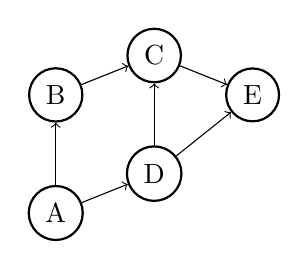
\begin{tikzpicture}[scale=0.5]
            \begin{scope}[every node/.style={circle,thick,draw}]
                \node (A) at (0,0) {A};
                \node (B) at (0,3) {B};
                \node (C) at (2.5,4) {C};
                \node (D) at (2.5,1) {D};
                \node (E) at (5,3) {E} ;
            \end{scope}

            \begin{scope}
                \path [->] (A) edge node {} (B);
                \path [->] (B) edge node {} (C);
                \path [->] (A) edge node {} (D);
                \path [->] (D) edge node {} (C);
                \path [->] (D) edge node {} (E);
                \path [->] (C) edge node {} (E);
            \end{scope}
            \end{tikzpicture}
        \caption{}
        \label{fig:graph}
    \end{figure}
    Il grafo di Figura \ref*{fig:graph} è descritto dalla coppia
    \begin{itemize}
        \item $N = \{A,B,C,D,E\}$
        \item $\to \,\,= \{(A,B), (A,D), (B,C), (D,C), (C,E), (D,E)\}$
    \end{itemize}
\end{example}
Un grafo è quindi un insieme di elementi (i \textit{nodi}) accoppiato con un insieme di relazioni tra questi elementi (gli \textit{archi} o \textit{rami}).\\
E' naturale associare questo concetto all'idea di percorso: ogni grafo è definito da un insieme di "luoghi" ed un insieme di "percorsi" che consentono di viaggiare
da un luogo ad un altro.\\
La seguente definizione sorge in modo spontaneo da questo punto di vista:
\begin{definition}
    Sia $G = (N, \to)$ un grafo. Siano $u,v \in N$. Diremo che \textit{$v$ è raggiungibile da $u$}, o in alternativa \textit{esiste un cammino da $u$ a $v$}, o ancora $u \to_t v$ (la $t$ in pedice è letta come \textit{transitivo}), se
    $\exists$ una sequenza $x_n \subset N$ finita di lunghezza $K : x_K = v, x_0 = u, x_n \to x_{n+1}$.
\end{definition}
L'esistenza di un cammino tra nodi fornisce un criterio immediato per suddividere un grafo in più pezzi. Riportiamo questo criterio come formulato in \cite{gentilini}:
\begin{definition}
    Sia $G = (N, \to)$ un grafo. Chiameremo \textit{grafo delle componenti fortemente connesse (CFC) di} $G$ il grafo $G^{CFC} = (N^{CFC}, \to^{CFC})$ se
    \begin{itemize}
        \item $N^{CFC} = \{C : C = \{m \in N : \forall n \in C, m \to_t n\}\}$
        \item $\to^{CFC} = \{(A,B) \in N^{CFC} \times N^{CFC} : A \neq B, \exists m \in A, n \in B : m \to n\}$
    \end{itemize}
\end{definition}
Segue immediatamente la seguente proprietà:
\begin{proposition}
    Sia $G^{CFC}$ il grafo delle CFC di un grafo $G$ generico. Allora $G^{CFC}$ è aciclico.
\end{proposition}
\begin{proof2}
    Suppongo per assurdo che in $G^{CFC}$ esista un ciclo, quindi è possibile partendo da un $A \in N^{CFC}$ ritornare ad $A$ seguendo un cammino che passa per un numero
    finito di nodi di $N^{CFC}$, che raggruppiamo nell'insieme $X \subset N^{CFC}$, con $A \not\in X$. Ma allora qualsiasi nodo
    $n \in N : (\exists B \in N^{CFC} \land n \in B \land B \in X)$ è raggiungibile da qualsiasi nodo di $A$. Quindi tutti i nodi inclusi nel ciclo devono appartenere alla
    stessa componente, ma questa deduzione è in contrasto con l'ipotesi.
\end{proof2}
\begin{example}
    \begin{figure}[t]
        \centering
        \begin{subfigure}{.49\textwidth}
          \centering
          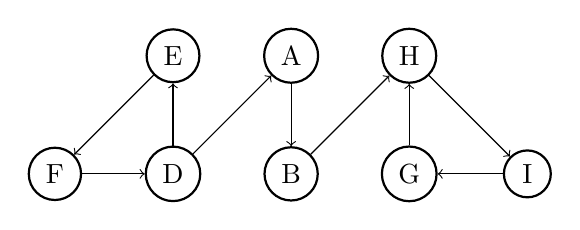
\begin{tikzpicture}[scale=0.5]
            \begin{scope}[every node/.style={circle,thick,draw}]
                \node (A) at (0,3) {A};
                \node (B) at (0,0) {B};

                \node (D) at (-3,0) {D};
                \node (E) at (-3,3) {E};
                \node (F) at (-6,0) {F};

                \node (G) at (3,0) {G};
                \node (H) at (3,3) {H};
                \node (I) at (6,0) {I};
            \end{scope}

            \begin{scope}
                \path [->] (A) edge node {} (B);

                \path [->] (E) edge node {} (F);
                \path [->] (F) edge node {} (D);
                \path [->] (D) edge node {} (E);

                \path [->] (G) edge node {} (H);
                \path [->] (H) edge node {} (I);
                \path [->] (I) edge node {} (G);

                \path [->] (D) edge node {} (A);
                \path [->] (B) edge node {} (H);
            \end{scope}
            \end{tikzpicture}
          \caption{}
        \end{subfigure}
        \begin{subfigure}{.49\textwidth}
          \centering
          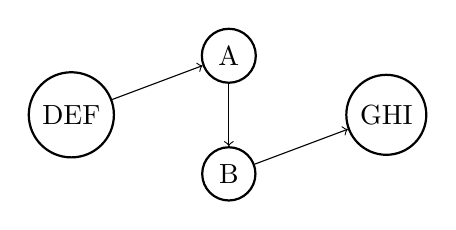
\begin{tikzpicture}[scale=0.5]
            \begin{scope}[every node/.style={circle,thick,draw}]
                \node (A) at (0,3) {A};
                \node (B) at (0,0) {B};

                \node (DEF) at (-4,1.5) {DEF};

                \node (GHI) at (4,1.5) {GHI};
            \end{scope}
                \path [->] (A) edge node {} (B);
                \path [->] (DEF) edge node {} (A);
                \path [->] (B) edge node {} (GHI);
            \begin{scope}

            \end{scope}
            \end{tikzpicture}
          \caption{}
        \end{subfigure}
        \caption{}
        \label{fig:graph_cfc}
    \end{figure}

    La figura \ref*{fig:graph_cfc}.a rappresenta un grafo generico, la figura \ref*{fig:graph_cfc}.b rappresenta il suo grafo delle componenti fortemente connesse associato.
\end{example}

\subsection{Applicazione dei grafi alla teoria degli insiemi}
\label{sec:graphs_sets}
Per motivi che risulteranno chiari in seguito risulta conveniente fornire un'interpretazione insiemistica della nozione di grafo vista sopra.
\begin{definition}
    Sia $G = (N, \to)$ un grafo direzionato. Sia $u \in N : \forall v \in N, u \to_t v$, cioè ogni nodo di $G$ è raggiungibile da $u$. Allora la terna $(N, \to, u)$ si dice \textit{accessible pointed graph}, o \textit{APG}.
\end{definition}
Se si associano la relazione di raggiungibilità $\to$ e la relazione di appartenenza $\in$, e se si interpreta ogni nodo come un insieme, ad ogni APG è possibile associare un unico insieme. Tuttavia ad ogni insieme si può associare più di un APG \cite{dovier}.
\begin{example}
    \begin{figure}[t]
        \centering
        \begin{subfigure}{.25\textwidth}
          \centering
          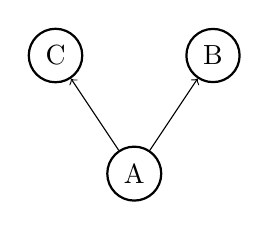
\begin{tikzpicture}[scale=0.5]
            \begin{scope}[every node/.style={circle,thick,draw}]
                \node (A) at (0,0) {A};
                \node (B) at (2,3) {B};
                \node (C) at (-2,3) {C};
            \end{scope}

            \begin{scope}
                \path [->] (A) edge node {} (B);
                \path [->] (A) edge node {} (C);
            \end{scope}
            \end{tikzpicture}
          \caption{}
        \end{subfigure}
        \begin{subfigure}{.15\textwidth}
            \centering
            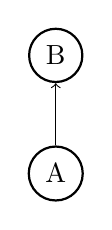
\begin{tikzpicture}[scale=0.5]
              \begin{scope}[every node/.style={circle,thick,draw}]
                  \node (A) at (0,0) {A};
                  \node (B) at (0,3) {B};
              \end{scope}

              \begin{scope}
                  \path [->] (A) edge node {} (B);
              \end{scope}
              \end{tikzpicture}
            \caption{}
          \end{subfigure}
        \begin{subfigure}{.15\textwidth}
          \centering
          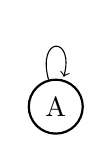
\begin{tikzpicture}[scale=0.5]
            \begin{scope}[every node/.style={circle,thick,draw}]
                \node (A) at (0,-1) {A};
            \end{scope}

            \begin{scope}
                \path [->] (A) edge [loop above] node {} (A);
            \end{scope}
            \end{tikzpicture}
          \caption{}
        \end{subfigure}
        \begin{subfigure}{.25\textwidth}
            \centering
            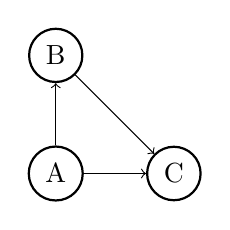
\begin{tikzpicture}[scale=0.5]
              \begin{scope}[every node/.style={circle,thick,draw}]
                  \node (A) at (0,0) {A};
                  \node (B) at (0,3) {B};
                  \node (C) at (3,0) {C};
              \end{scope}

              \begin{scope}
                  \path [->] (A) edge node {} (B);
                  \path [->] (B) edge node {} (C);
                  \path [->] (A) edge node {} (C);
              \end{scope}
              \end{tikzpicture}
            \caption{}
          \end{subfigure}

        \caption{}
        \label{fig:graph_set}
    \end{figure}

    Il grafo in figura \ref*{fig:graph_set}.a e quello in \ref*{fig:graph_set}.b rappresentano l'insieme $A = \{\emptyset\}$.
    Il grafo in figura \ref*{fig:graph_set}.c rappresenta l'insieme $A = \{A\}$.
    Il grafo in figura \ref*{fig:graph_set}.d rappresenta l'insieme $A = \{\emptyset, \{\emptyset\}\}$
\end{example}

\subsection{Bisimulazione}
\begin{definition}
    Siano $G_1 = (N_1, E_1), G_2 = (N_2, E_2)$ due grafi. Diremo che $G_1, G_2$ sono \textit{bisimili} (come in \cite{dovier}) rispetto alla relazione binaria $b$ su $N_1, N_2$ se $\forall u \in N_1, v \in N_2$ valgono congiuntamente le seguenti condizioni
    \begin{itemize}
        \item $\forall u' \in N_1 : u \to u', u b v \implies \,\exists v' \in N_2 : (u' b v' \land v \to v')$
        \item $\forall v' \in N_2 : v \to v', u b v \implies \,\exists u' \in N_1 : (u' b v' \land u \to u')$
    \end{itemize}
\end{definition}
Se per una determinata coppia di grafi esiste almeno una bisimulazione che li lega, possiamo dedurre che i nodi dei due grafi mostrano un comportamento simile.
Questo concetto verrà chiarito in seguito, per ora forniamo solamente la seguente definizione:
\begin{definition}
    Siano $G_1 = (N_1, E_1, v_1), G_2 = (N_2, E_2, v_2)$ due APG. Diremo che sono \textit{bisimili} se $\exists$ una bisimulazione $b$ su $G_1, G_2 : v_1 b v_2$.
\end{definition}
Per introdurre i risultati che verranno presentati in seguito risulta utile definire la bisimulazione su un unico grafo:
\begin{definition}
    Sia $G = (N, \to)$ un grafo, e $b$ una relazione binaria su $N$. Diremo che $b$ è una \textit{bisimulazione} se $\forall u,v \in N$ valgono congiuntamente le seguenti condizioni
    \begin{itemize}
        \item $\forall u' \in N : u \to u', u b v \implies \,\exists v' \in N : (u' b v' \land v \to v')$
        \item $\forall v' \in N : v \to v', u b v \implies \,\exists u' \in N : (u' b v' \land u \to u')$
    \end{itemize}
\end{definition}
Proponiamo ora un risultato che consentirà di considerare più generali di quanto sembrino in apparenza alcuni risultati presentati nel seguito del lavoro.
\begin{theorem}
    Sia $b$ una bisimulazione sul grafo $G$. La sua chiusura riflessiva, simmetrica o transitiva è ancora una bisimulazione su $G$.
\end{theorem}
\begin{proof2}
    Consideriamo separatamente le tre relazioni $b_r, b_s, b_t$, rispettivamente la chiusura riflessiva, simmetrica e transitiva:
    \begin{itemize}
        \item[$b_r$] Per definizione $b \subset b_r$, quindi è sufficiente dimostrare che $b_r$ è una bisimulazione quando gli argomenti $u,v \in N$ non sono distinti.\\
        Sia $u \in N$. Chiaramente per definizione di $b_r$ si ha $u b_r u$. Se $\exists u' \in N : u \to u'$ allora (sempre per definizione di $b_r$) si ha $u' b_r u'$.
        \item[$b_s$] Per definizione $b \subset b_s$, quindi è sufficiente dimostrare che $b_s$ è una bisimulazione quando per gli argomenti $u,v \in N$ si ha $u b v$ ma non $v b u$.\\
        Sia $(u,v) \in N \times N$. Allora
        \begin{center}
            $u b_s v \implies u b v \lor v b u$
        \end{center}
        Suppongo ad esempio che $v b u$.
        \begin{align*}
            &\implies \forall v' \in N : (v \to v') \,\,\exists u' \in N : (u \to u' \land v' bu')\\
            &\implies u' b_s v'
        \end{align*}
        e
        \begin{align*}
            &\implies \forall u' \in N : (u \to u') \,\,\exists v' \in N : (v \to v' \land v' bu')\\
            &\implies u' b_s v'
        \end{align*}
        cioè sono dimostrate le due condizioni caratteristiche della bisimulazione.\\
        La dimostrazione è analoga se $u b v$.
        \item[$b_t$] Per definizione $b \subset b_t$, quindi è sufficiente dimostrare che $b_t$ è una bisimulazione quando per gli argomenti $u,v,z \in N$ si ha $u b v$, $v b z$ ma non $u b z$.\\
        Sia $(u,v,z) \in N \times N \times N$ con questa proprietà. Allora $\forall u' \in N : u \to u' \implies \exists v' \in N : v \to v' \land u' b v'$. Inoltre $\exists z' : z \to z' \land v' b z'$.\\
        Riordinando si ha $u' b v', v' b z'$. Allora per definizione di $b_t, \, u' b_t z'$.\\
        In modo speculare si ottiene la seconda condizione caratteristica della bisimulazione.
    \end{itemize}
\end{proof2}
Da questa proposizione si deduce il seguente corollario, che risulta dall'applicazione iterativa delle tre chiusure viste in precedenza:
\begin{corollary}
    Ad ogni bisimulazione $b$ è possibile associare una bisimulazione $\widetilde{b} : b \subset \widetilde{b} \,\,\land\,\, \widetilde{b}$ è una relazione di equivalenza.
    \label{cor:bisimulation_eqrel}
\end{corollary}
Concludiamo la parte relativa ai risultati generali sulla bisimulazione con la seguente proposizione, che sarà utile in seguito
\begin{proposition}
    Siano $b_1, b_2$ due bisimulazioni su $G_1, G_2$. Allora $b = b_1 \cup b_2$ è ancora una bisimulazione.
    \label{obs:bisimulation_union}
\end{proposition}
\begin{proof2}
    Siano $u,v : u b v$. Sia $u' : u \to u'$. Allora deve essere $u b_1 v \lor u b_2 v$. Ma quindi $\exists v' : (v \to v' \land u' b_{1|2} v')$.
\end{proof2}

\subsubsection{Bisimulazione massima}
\label{sec:bisi_max}
Definiamo ora il concetto di \textit{bisimulazione massima}, che gioca un ruolo chiave nella risoluzione dei problemi considerati in questo elaborato.
\begin{definition}
    Diremo che una bisimulazione $b_M$ su $G_1, G_2$ è \textit{massima} se $\forall b : "b$ è una bisimulazione su $G_1, G_2$" si ha $u b v \implies u b_M v \,\,\,\forall a \in N_1, b \in N_2$.
\end{definition}
Naturalmente la bisimulazione massima dipende dai due grafi presi in esame. Possiamo dedurre alcune caratteristiche in modo molto semplice:
\begin{proposition}
    Valgono le seguenti proprietà:
    \begin{enumerate}
        \item La bisimulazione massima su due grafi $G_1,G_2$ è unica
        \item La bisimulazione massima è una relazione di equivalenza
    \end{enumerate}
\end{proposition}
\begin{proof2}
    Le proprietà seguono banalmente dal Corollario \ref*{cor:bisimulation_eqrel} e dall'Osservazione \ref*{obs:bisimulation_union}.
    \begin{enumerate}
        \item Suppongo per assurdo che esistano due bisimulazioni massime $b_{M_1}, b_{M_2}$. La loro unione è ancora una bisimulazione, che è "più massima" delle supposte bisimulazioni massime.
        \item Se per assurdo la bisimulazione massima non fosse una relazione di equivalenza, potremmo considerare la sua chiusura riflessiva, simmetrica e transitiva, che sarebbe "più massima" ed anche una relazione di equivalenza.
    \end{enumerate}
\end{proof2}
Naturalmente il concetto di \textit{bisimulazione massima} può essere definito anche su unico grafo $G$. Questo caso si rivelerà di grande interesse nel seguito. Per
ora dimostriamo il seguente risultato:
\begin{theorem}
    Sia $G$ un grafo (finito). Allora $\exists b_M$ la bisimulazione massima su $G$.
\end{theorem}
\begin{proof2}
    Può esistere solamente un numero finito di relazioni binarie su $G$, e questo numero fornisce un limite superiore al numero massimo di bisimulazioni su $G$.
    Allora possiamo considerare l'unione di questo numero finito di bisimulazioni, che sarà chiaramente la bisimulazione massima.
\end{proof2}

\subsubsection{Interpretazione insiemistica della bisimulazione}
Il seguente teorema è la prova che la bisimulazione può essere utilizzata per verificare l'uguaglianza tra insiemi rappresentati da due APG differenti:
\begin{theorem}
    Due APG sono bisimili $\iff$ rappresentano lo stesso insieme.
    \label{theo:bisi_iff_eqsets}
\end{theorem}
\begin{proof2}
    Da dimostrare...
\end{proof2}
Tenendo conto di quanto affermato nella sezione \ref*{sec:graphs_sets}, il Teorema \ref*{theo:bisi_iff_eqsets} dimostra che la bisimulazione può sostituire la
relazione di uguaglianza tra insiemi quando questi sono rappresentati da degli APG \cite{dovier}.\\
Dopo questa considerazone, risulta naturale definire il seguente concetto:
\begin{definition}
    Sia $b$ una bisimulazione su $G$ che sia anche una relazione di equivalenza. Definiamo un nuovo grafo $G_b = (N_b, \to_b)$ come in \cite{gentilini}, che chiameremo \textit{contrazione rispetto alla bisimulazione} $b$ \textit{di} $G$:
    \begin{itemize}
        \item $N_b = \{A = \{m \in N : \forall n \in A, m b n\}\}$
        \item $[m]_b \to_b [n]_b \iff \exists c \in [n]_b : m \to c$
    \end{itemize}
    Risulta conveniente definire la \textit{classe del nodo} $a$ rispetto alla bisimulazione $b$, con la notazione $[a]_b$ come il nodo di $N_b$ a cui appartiene il nodo $a$.
    \label{def:bisi_contraction}
\end{definition}
La Definizione \ref*{def:bisi_contraction} è di fondamentale importanza per la seguente osservazione:
\begin{proposition}
    Sia $G$ un grafo, e sia $G_b$ come nella Definizione \ref*{def:bisi_contraction}, per una bisimulazione $b$ qualsiasi. Allora $G, G_b$ sono bisimili.
    \label{prop:bisi_cont_bisi}
\end{proposition}
\begin{proof2}
    Sia $\equiv \,\,\subset N \times N_b$ la relazione binaria definita come segue:
    \begin{gather*}
        m \equiv M \iff M = [m]_b
    \end{gather*}
    Vogliamo dimostrare che tale relazione è una bisimulazione su i grafi $G, G_b$.\\
    Supponiamo che $x \equiv X$, e che $x \to y$ per qualche $y \in N$. Chiamiamo $Y \coloneqq [y]_b$. Allora, per la Definizione \ref*{def:bisi_contraction}, si ha $X \to Y$. Inoltre vale banalmente $y \equiv Y$.\\
    Per dimostrare la seconda condizione caratteristica della bisimulazione, supponiamo che $x \equiv X$, e che $X \to Y$ per qualche $Y \in N_b$. Sempre per la Definizione \ref*{def:bisi_contraction} deve esistere un $y \in Y : (y \equiv Y \land x \to y)$.
\end{proof2}
La Proposizione \ref*{prop:bisi_cont_bisi} ha una conseguenza ovvia, che risulta evidente per il Teorema \ref*{theo:bisi_iff_eqsets}:
\begin{corollary}
    Sia $b$ una bisimulazione che sia anche una relazione di equivalenza. Allora l'APG $(G, v)$ e l'APG $(G_b, [v]_b)$ rappresentano lo stesso insieme.
\end{corollary}
Quindi risulta naturale sfruttare le proprietà della bisimulazione per minimizzare la rappresentazione di insiemi, considerando che è sufficiente una bisimulazione sulla rappresentazione iniziale per ottenere una rappresentazione equivalente. Definiamo una relazione d'ordine sulle rappresentazioni:
\begin{definition}
    Diremo che la rappresentazione $(G_a, v_a)$ di un insieme è \textit{minore} della rappresentazione equivalente $(G_b, v_b)$ se $\#N_a < \#N_b$.\\
    Diremo che una rappresentazione è \textit{minima} se non esiste un'altra rappresentazione minore.
\end{definition}
\begin{observation}
    La \textit{contrazione per bisimulazione} di un grafo ha sempre un numero di nodi minore o uguale di quello del grafo iniziale.
\end{observation}
Concludiamo la sezione con il seguente risultato, che stabilisce in modo univoco la bisimulazione prescelta per minimizzare la rappresentazione di un dato insieme:
\begin{theorem}
    Sia $(G,v)$ un APG rappresentante un insieme. Sia $b_M$ la bisimulazione massima su $(G,v)$. Allora la contrazione per bisimulazione indotta da $b_M$ su $(G,v)$ fornisce la rappresentazione minima dell'insieme.
\end{theorem}
\begin{proof2}
    Suppongo per assurdo che esista una bisimulazione $b_N$ su $(G,v)$ che fornisce una contrazione avente un numero di nodi strettamente inferiore alla contrazione indotta da $b_M$. Ma questo implica che esistono almeno due nodi di $G$ che sono in relazione secondo $b_N$ e non secondo $b_M$. Chiaramente questa deduzione è in contrasto con il fatto che $b_M$ è la bisimulazione massima.\\\\
    Suppongo per assurdo che, dopo la contrazione indotta da $b_M$, sia possibile trovare una nuova bisimulazione $b_O$ su $(G_{b_M}, [v]_{b_M})$ che induca una contrazione avente un numero di nodi strettamente inferiore a quello di $(G_{b_M}, [v]_{b_M})$. Chiaramente $b_O \subset N_{b_M} \times N_{b_M}$.\\
    Definisco una nuova bisimulazione $b_{\widetilde{M}} \subset N \times N$ tale che
    \begin{gather*}
        x b_{\widetilde{M}} y \iff (x b_M y \lor [x]_{b_M} b_O [y]_{b_M})
    \end{gather*}
    Per definizione di bisimulazione massima bisogna avere $b_{\widetilde{M}} \subset b_M$, quindi non è possibile che la contrazione indotta da $b_O$ sia una rappresentazione minore di quella indotta da $b_M$.
\end{proof2}
